%%This is a very basic article template.
%%There is just one section and two subsections.
\documentclass{article}
\usepackage[latin1]{inputenc} %coding of writteninput %latin1 allows for Umlaute
\usepackage[T1]{fontenc}%vectorized fonts (cm-super package)
\usepackage[german]{babel}%some specifics of the german language
\usepackage{amsfonts, amsmath, amsthm, amssymb, mathabx, paralist}
 \setlength{\parindent}{0em} 
  \usepackage{listings}
\usepackage{geometry}
  \geometry{a4paper, top=25mm, left=20mm, right=15mm, bottom=20mm, headsep=10mm, footskip=12mm}
 \usepackage{rotating} 
 %Decisiontree
 \usepackage{tikz,forest}
\usetikzlibrary{arrows.meta,arrows,shadows,positioning,decorations.pathreplacing}
\pgfdeclarelayer{background}
\pgfdeclarelayer{foreground}
\pgfsetlayers{background,main,foreground}
\usepackage{float}
\usepackage{enumitem}



  
\usepackage{graphicx} 

\usepackage{verbatim}%f�r txt datei

\usepackage{color} %red, green, blue, yellow, cyan, magenta, black, white
\definecolor{mygreen}{RGB}{28,172,0} % color values Red, Green, Blue
\definecolor{mylilas}{RGB}{170,55,241}

\usepackage[section]{placeins}

\begin{document}

\subsection*{Rapidminer}
For simplicity a powerful software system with a variety of different ways for clustering analysis, called Rapidminer Studio, is used to find correlations between spatio temporal data points. It enables to graphically form a pipeline from our spatio temporal input data to a concrete clustering by composing small blocks called \textbf{operators}. The first approach is to simply retrieve the base data from Medell�n and feed it into a clustering operator which uses K-means. 

\subsubsection*{Corrupted Data}
The first visible thing is that the data is corrupted, i. e. there are missing values for some data points, which are not allowed for the clustering operators. To fix this issue the missing values are replaced with the average value of the respective attribute. Since the data has both categorical and numerical values, the mixed euclidian distance is used as similarity measure to calculate the difference between two data points with both numerical and categorical attributes.

\begin{enumerate}
	
	\item Exponential distribution of travels regarding traveling distance\\\\
	
	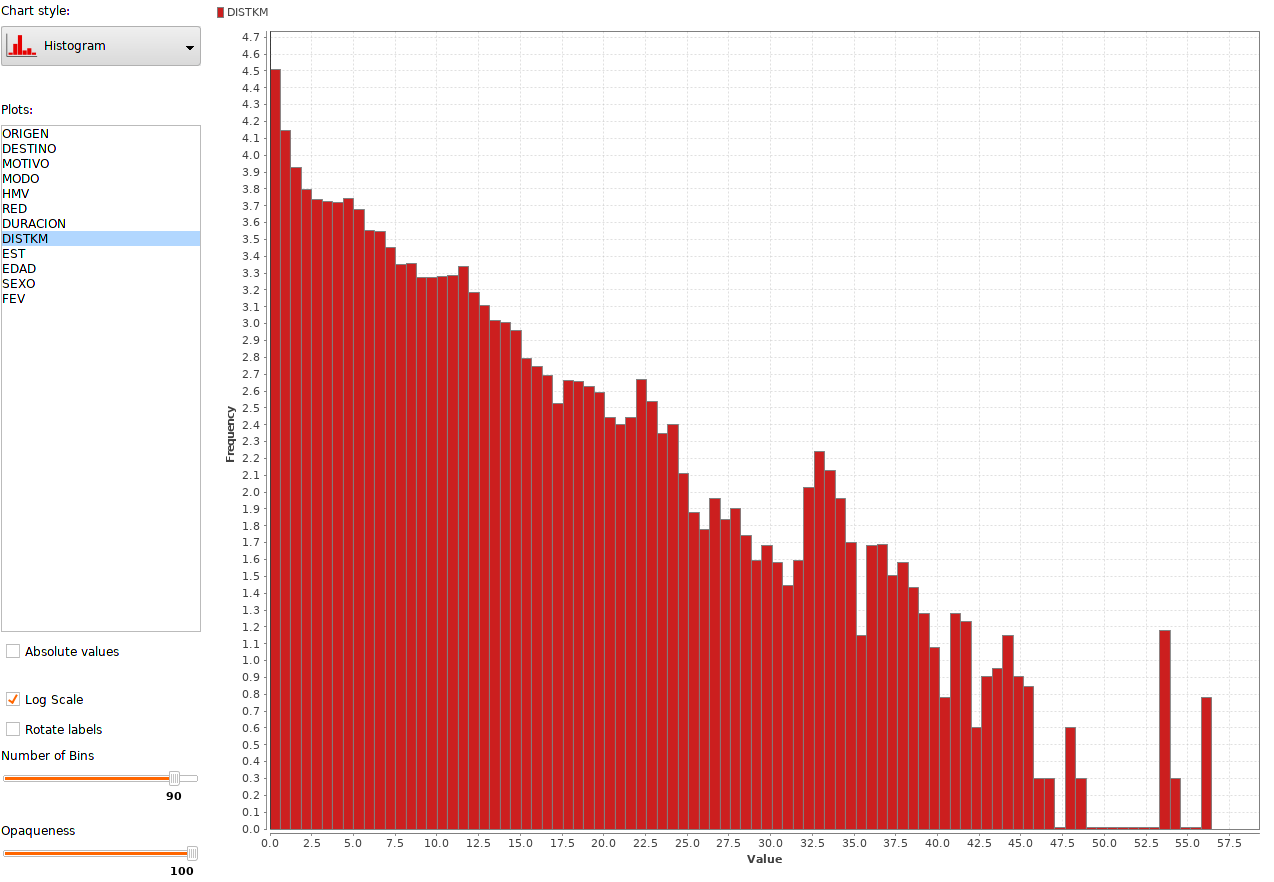
\includegraphics[width=0.5\textwidth]{data_findings/exponential distr.png}
\end{enumerate}

\end{document}













